\documentclass[11pt]{ecsarticle}
%\usepackage[nodayofweek]{datetime}
\usepackage{natbib} 
\usepackage{graphicx}
\usepackage{caption}
\usepackage{subcaption}



\title{COMP6026 - Assignment 2 - Group Selection}
\authors{Henry Lovett - hl13g10}
\begin{document}
\maketitle
 
\section{Introduction}

In an evolutionary sense, being selfish is advantageous \cite{} as an individual can reap the benefits of being in a group without any contribution.
A basic example of this is the Prisoner's Dilemma \cite{}.
However, in nature, cooperation is common. 
This then raises the question of why cooperation exists. 

In \cite{powers2007individual}, a situation was set up with individuals that are selfish and cooperative. 
Each individual also has a preference of being in a small or large group. 
Resources were allocated to the groups and the population increased depending on the amount of resources the genotype had. 
Selfish individuals had a higher growth, but higher consumption of the resource than the cooperative.
A small group had less resources per captia than the large group.

By doing this, it was shown that the genotype of small cooperators flourished and became the only genotype in the population. 

%Describe paper/experiment.
%Game theory game - defectors win CITE

This paper discusses the reimplementation of the experiment \cite{powers2007individual} and a comparison of results in sections \ref{sc:reimplementation} and \ref{sc:reimp:results}.
An extension to this work is covered in section \ref{sc:extension}, the results of which are shown in \ref{sc:results} and section \ref{sc:conclusion} concludes the paper.


\section{Reimplementation}\label{sc:reimplementation}
\begin{itemize}
 \item Initialise
 \item for number of generations:
 \begin{itemize}
  \item Make groups
  \item for timesteps:
  \begin{itemize}
   \item Allocate resources
   \item Grow populatiosn
  \end{itemize}
  \item Reform migrant pool
  \item Scale migrant pool
 \end{itemize}

\end{itemize}


%How individuals were represented
This experiment used individuals with two genotypes, giving four possible combinations of individual.
The genotypes were whether the individual prefered small or large groups, and whether it was selfish or cooperative.
The four possible combintation therefore were: cooperative \& small, selfish \& small, cooperative \& large, selfish \& large. 

In the reimplementation, an individual was not explicitly represented. 
Instead, a list of four values was used to store the total number of each genotype. 
This was used for both the migrant pool and the groups. 

Initialisation was done exactly propotionatly. Each genotype was assigned $N / 4$ number of individuals.

%Group allocation
During each generation, the migrant pool was split down into as many small groups as possible.
Individuals were split into either small or large groups depending on their preference in their genotype.
Groups were made to represent the proportions of the global migrant pool. 
Only full groups were allowed and any members left over from group allocation were removed from the population. 
These groups were then allocated resources and allowed to grow. 

%Resource equation \& explanation
Resources were allocated to each genotype propotionatly, depending on their genotype.
This was done using equation \eqref{eq:resource}. 
It is biased to allocate more resource to the selfish genotype ($0.02 \times 0.2 > 0.018 \times 0.1$). 
R also changes depending on the group size - small groups have limited resources to encourage cooperation, and large groups have more resource per captia.
\begin{equation}
 r_i = \frac{ n_i . G_i . C_i }{\sum\limits_j (n_j . G_j . C_j )} . R 
 \label{eq:resource}
\end{equation}

%Growth equation \& explanation
Once the resources are allocated, the groups are then grown. 
The new population size is calculated by three terms, seen in equation \ref{eq:growth}. 
The first is the current size and the third is a constant death rate to all genotypes.
The middle term uses the resouces allocated and the consumption rate of the genotype.
As the consumption for a cooperative genotype is lower, this is biased to grow the cooperators more.
\begin{equation}
 n_i (t + 1) = n_i (t) + \frac{r_i}{C_i} - K.n_i (t)
 \label{eq:growth}
\end{equation}

\begin{table}
 \begin{tabular}{|c|c|}\hline
  Cooperative consumption rate, $C_c$	&	$0.1$		\\ \hline
  Selfish consumption rate, $C_s$	&	$0.2$		\\ \hline
  Cooperative growth rate, $G_c$	&	$0.018$		\\ \hline
  Selfish growth rate, $G_s$		&	$0.02$		\\ \hline
  Population size, $N$			&	$4000$		\\ \hline
  Small group size, $N\_small$		&	$4$		\\ \hline
  Large group size, $N\_large$		&	$40$		\\ \hline
  Number of generations, $N$		&	$120$		\\ \hline
  Number of timesteps, $t$		&	$4$		\\ \hline
  Resource for small groups, $R_{small}$&	$4$		\\ \hline
  Resource for large groups, $R_{large}$&	$50$		\\ \hline
  Death rate, $K$			&	$0.1$		\\ \hline
 \end{tabular}
 \caption{Parameters used in the reimplementation}
 \label{table:params}
\end{table}

\section{Comparison of results}\label{sc:reimp:results}
\begin{figure}
        \centering
        \begin{subfigure}[b]{0.4\textwidth}
                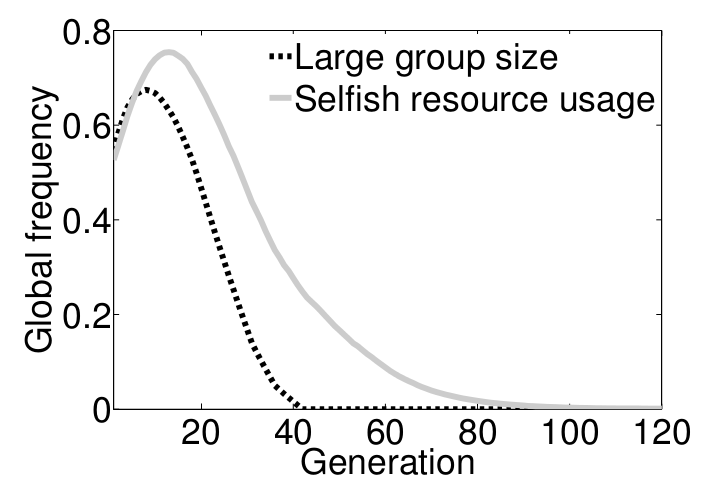
\includegraphics[width=0.4\textwidth]{orig_a.png}
                \caption{The original results from \cite{powers2007individual}.}
                \label{fig:orig:A}
        \end{subfigure}%
        ~ %add desired spacing between images, e. g. ~, \quad, \qquad etc.
          %(or a blank line to force the subfigure onto a new line)
        \begin{subfigure}[b]{0.4\textwidth}
                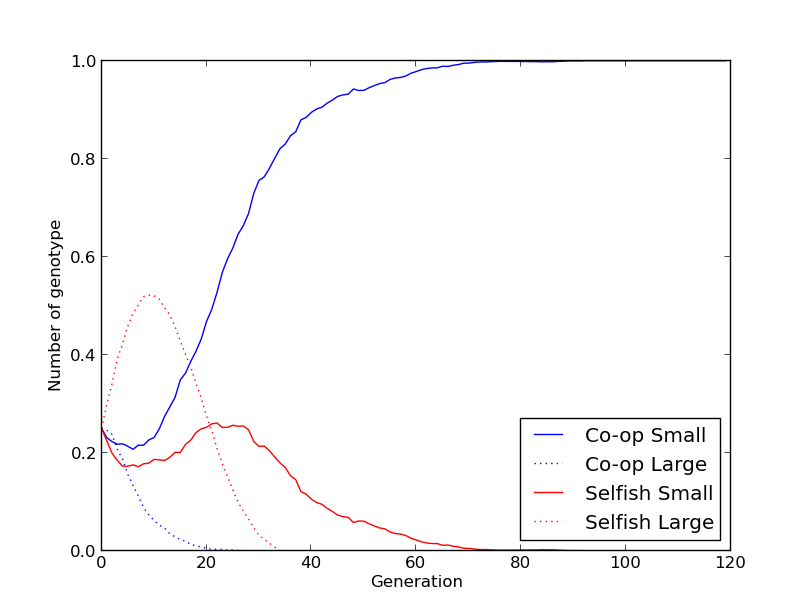
\includegraphics[width=0.4\textwidth]{Code2/fig1.png}
                \caption{Reproduced results}
                \label{fig:orig:B}
        \end{subfigure}
        \caption{Average environment and strategy through time.}\label{fig:A}
\end{figure}

\begin{figure}
        \centering
        \begin{subfigure}[b]{0.4\textwidth}
                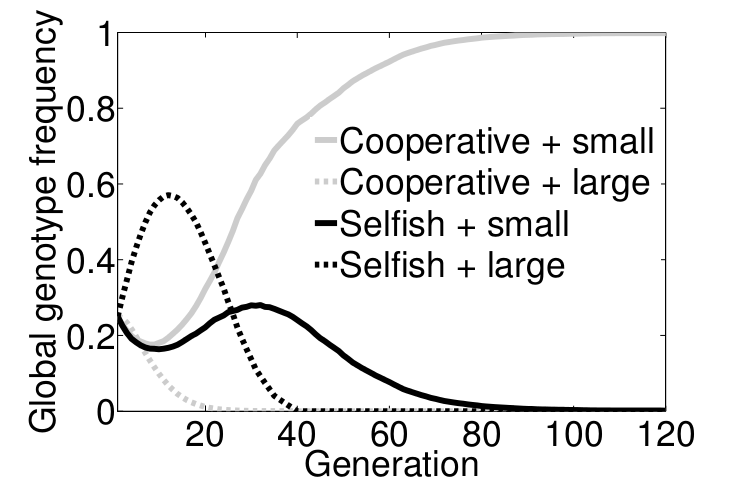
\includegraphics[width=\textwidth]{orig_b.png}
                \caption{The original results from \cite{powers2007individual}.}
                \label{fig:rep:A}
        \end{subfigure}%
        ~ %add desired spacing between images, e. g. ~, \quad, \qquad etc.
          %(or a blank line to force the subfigure onto a new line)
        \begin{subfigure}[b]{0.4\textwidth}
                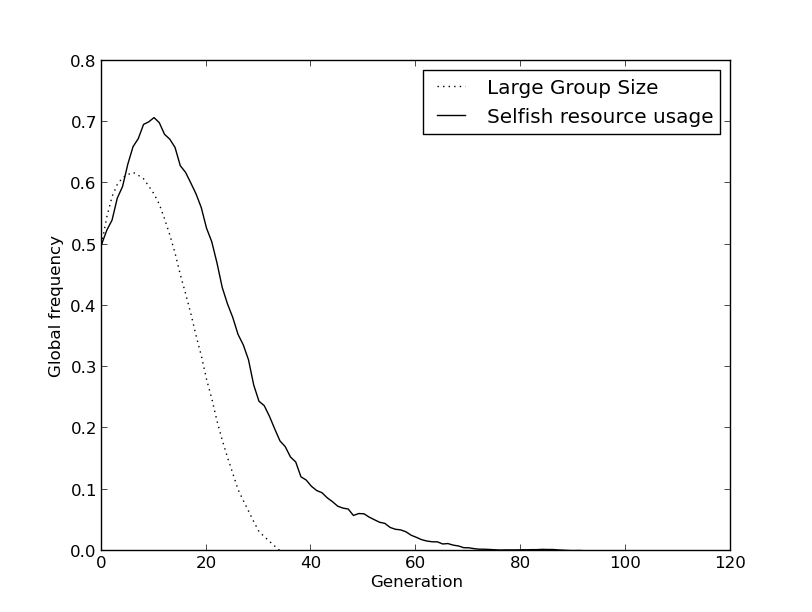
\includegraphics[width=\textwidth]{Code2/fig2.png}
                \caption{Reproduced results.}
                \label{fig:rep:B}
        \end{subfigure}
        \caption{Change in genotype frequencies over time.}\label{fig:B}
\end{figure}

The reproduced results were found to be very close to the original data. 
Figure \ref{fig:B} shows the proportion of each genotype in the population.
In both graphs, the cooperators in the large group get immediately out competed by the selfish, and are then pushed to extinction.
The numbers of large selfish then begin to diminish and both small genotypes increase before the cooperative small genotype excells and results in being the entire of the population.
The population reached a steady state by 100 generations.

Figure \ref{fig:A} shows the proportions of the strategies. 
Both results show that the large populations reach 0 first and the selfish gene takes a little longer to be removed from the population.

The results obtained from the extension proved to be a very close replication to the original data, and therefore can be used for an extension of this work.

\section{Extension}\ref{sc:extension}

\section{Results}\ref{sc:results}

\section{Conclusion}\ref{sc:conclusion}


\bibliographystyle{apalike}
\bibliography{bibliography}
 
\end{document}
